\subsection{Translational Forces induced by the Static Field}
\label{sec:translationalForceBG}

In the \gls{mri} environment, the dominant safety concern for non-ferromagnetic objects arises not at isocenter, where the static field $ B_0  $ is uniform and $  \frac{dB_0}{dz} \approx 0  $, but in the fringe field region outside the bore, where strong spatial gradients exist.

Consider a simple pendulum with a metallic object at its end. This object is free to swing along the z-axis of an \gls{mri}. A static magnetic field along that same axis is then applied. The pendulum would be pulled towards the magnet with a force $F_m$ until it reaches equilibrium with its weight $mg$ and tension $T_s$. Figure \ref{fig:astm_diagram} shows a complete free body diagram.

\begin{figure}[htb!]
	\centering
	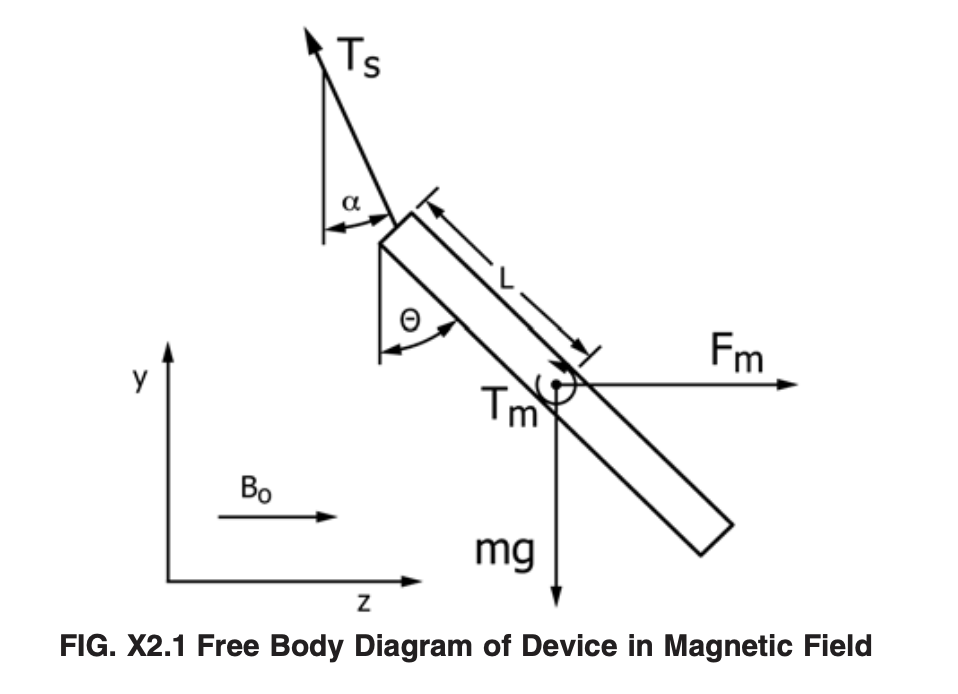
\includegraphics[width=0.4\textwidth]{Assets/astm_diagram.png}
	\caption[Free-body diagram of a metallic pendulum object in a static MRI magnetic field]{Free-body diagram of device in magnetic field (adapted from ASTM F2052-15 \cite{astmF2052}, Appendix X2).}
	\label{fig:astm_diagram}
\end{figure}

From Newton's laws at equilibrium point, the magnetic force can be found by measuring the angular deflection $\alpha$ such that 

\begin{equation}
	F_m = mg tan(\alpha). 
	\label{eq:Newton_translationalForce}
\end{equation}

Noting that this solution is independent of the point of attachment of the string and holds if the center of magnetic force does not coincide with the center of mass \cite{astmF2052}. On the other hand, by using Equations and \ref{eq:force} \ref{eq:magnitudemoment}, the magnetic force also is

\begin{equation}
	F_m =  \frac{\chi_m V}{\mu_0} B_0 \frac{dB_0}{dz}
	\label{eq:translationalForce}
\end{equation}

By comparing the magnetic force to the gravitational force ($F_g = m g$) the safety condition arises. If the device deflects less than $\alpha$ 45$^\circ$, then the magnetically induced deflection force is less than the force on the device due to its weight \cite{astmF2052}. This formulation explains why the measured deflection angle $\alpha$ (and thus $F_m$) depends not on $\chi$ or $B_0$ independently, but on their product. Practically, this insight justifies the lab methodology. Although magnets in our lab, a solenoid or neodymium magnets, generate small magnetic fields (only about 20 to 300 Gauss), we can use samples with proportionaly larger $\chi_m$ to replicate clinically relevant force-to-weight ratios ($F_m / F_g$). An estimation for the expected $\chi_m$ can be found on appendix \ref{app:scaling} and summarized in table \ref{tab:chi_scaling}.

%From equation (\ref{eq:forFit}), 
The measurable magnetic deflection depends on the ratio between the mechanical term and the magnetic force term. To reproduce the same deflection, 1 cm, at laboratory field strengths much smaller than those in MRI systems, the product must be preserved. Because $B_0 \nabla B_0 \propto B^2_0$ for a geometrically similar field, scaling the field down by a factor of  $10^2$ requires increasing the sample’s effective susceptibility by roughly $10^4$ to maintain the same mechanical response.

\begin{table}[htb]
	\centering
	\caption[Representative susceptibility scaling for laboratory solenoid fields.]{Values indicate the minimum magnetic susceptibility required to produce a measurable angular deflection (~1 cm over 1 m) under reduced field conditions (30–300 G and 3T), assuming a material density of ~7000 $kg/m^3$.}
	\label{tab:chi_scaling}
	\begin{tabular}{|c|c|c|c|}
		\hline
		$B_0$ (T) & $B\nabla B$ (T$^2$/m) & $\chi/\rho$ (m$^3$/kg) & $\chi_m$ (-) \\
		\hline
		$3.0 \times 10^{-3}$ & $1.707 \times 10^{-5}$ & $7.21 \times 10^{-3}$ & $5.05 \times 10^{\phantom{-}1}$ \\
		$3.0 \times 10^{-2}$ & $1.707 \times 10^{-3}$ & $7.21 \times 10^{-5}$ & $5.05 \times 10^{-1}$ \\
		$3.0 \times 10^{\phantom{-}0}$  & $1.707 \times 10^{\phantom{-}1}$  & $7.21 \times 10^{-9}$ & $5.05 \times 10^{-5}$ \\
		\hline
	\end{tabular}
\end{table}

For typical solenoids producing 30–300 G, the factor of $\chi_m/\rho$ spans from approximately one hundred-thousandth to one-thousandth of that found in ferromagnetic materials. Consequently, to appropriately mimic translational forces under these laboratory conditions, a realistic value of $\chi_m$ for a substitute should lie between one and ten. For example, a nonmagnetic stainless steel wire ($\chi_m \approx 10^{-4}$) might show a magnetic force of 30\% of the object's weight, whereas ferromagnetic metals like nickel can exceed two million percent. That is more than enough to become dangerous projectiles unless restrained \cite{aboyewa2021,Woods2021_MRIdisplacement,panych2018}.

